\documentclass[a4paper,12pt]{article}

\usepackage[margin=0.75in]{geometry} 
\usepackage{url}
\usepackage{graphicx}

\graphicspath{/images/}

\begin{document}	
\title{Software Architecture Assignment Semester One}
\author{Henry Senior\\@00454779}
\date{December 2017}

\maketitle

\section*{Introduction}
When designing and creating software, it is common to think about the end user experience. However, it is also important to consider what software development consultant Kevlin Henney describes as the, \textit{``Programmer Experience''}. \cite{FizzBuzz}. This refers to the readability, maintainability, and reusability of the source code. He argues that if programmers cannot understand the source code, then they cannot use it effectively. However, as Gamma \textit{et al} (commonly known as The Gang of Four or GoF) state \textit{`Designing object-oriented software is hard, and designing reusable object-oriented software is even harder.'} \cite{GoF-Book}. This report both explains and evaluates the design decisions taken during the creation of my educational game, Bug Busters, and how they impacted on the; usability, efficiency, reliability, maintainability, and reusability of the source code. 

\section*{Design}
\subsection*{Use Case Diagrams}
Use case diagrams provide a way of representing the scenarios that are connected by a common goal \cite{UML-Distilled}. Creating use case diagrams is a key part of Responsibility Driven Design as it allows the system architect to move from an abstract brief such as \textit{`a tower defence game where the user plays as the immune system'} to a more concrete understanding of what the final product should offer. 
\begin{figure}[h!]
	\begin{center}
		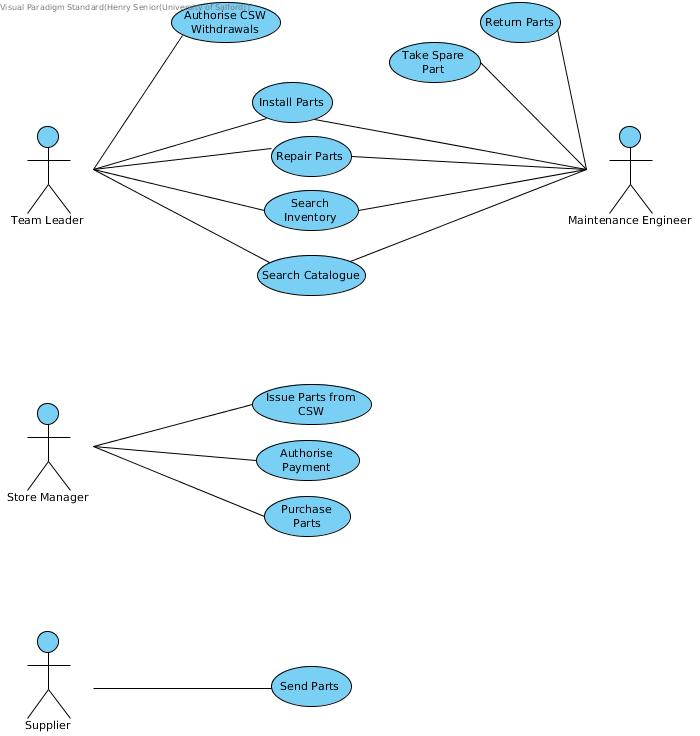
\includegraphics[width=7cm, origin=h]{images/Use-Case.jpg}
		\\
		\caption{A use case diagram drawn in Visual Paradigm}
	\end{center}
\end{figure}
\\
Creating a use case diagram enabled me to focus on the key features of the game. As it was a tower defence game, many of the key use cases revolve around the user's interaction with the towers. The fun of tower defence comes from selecting where you think certain towers would be best placed for defence. It was a natural decision to ensure the user could purchase towers and select where they are placed throughout the map. It also became clear that users should be able to upgrade towers to a certain level. To increase replay value and offer different levels of difficulty, the decision was taken to offer a selection of maps.


\subsection*{Software Components and Sequence Diagrams}
After creating a use case diagram it was possible to decide on the main modules that would make up the game. It became clear that there would be different screens, and these would be grouped into one module. In order to decouple the user interface of the game screen from the screen itself and increase the cohesion the different parts of the user interface have with the other modules, the individual components that make up the user interface were grouped into a second component. The third component would house all the classes that make up the towers and the fourth component would be made up of the pathogen classes. 
\\
Sequence Diagrams are especially good at showing the flow between different components when a use case is being executed. A sequence diagram has been used to show the dynamic interaction between software components for the `select map' use case. 
\begin{figure}[h!]
	\begin{center}
		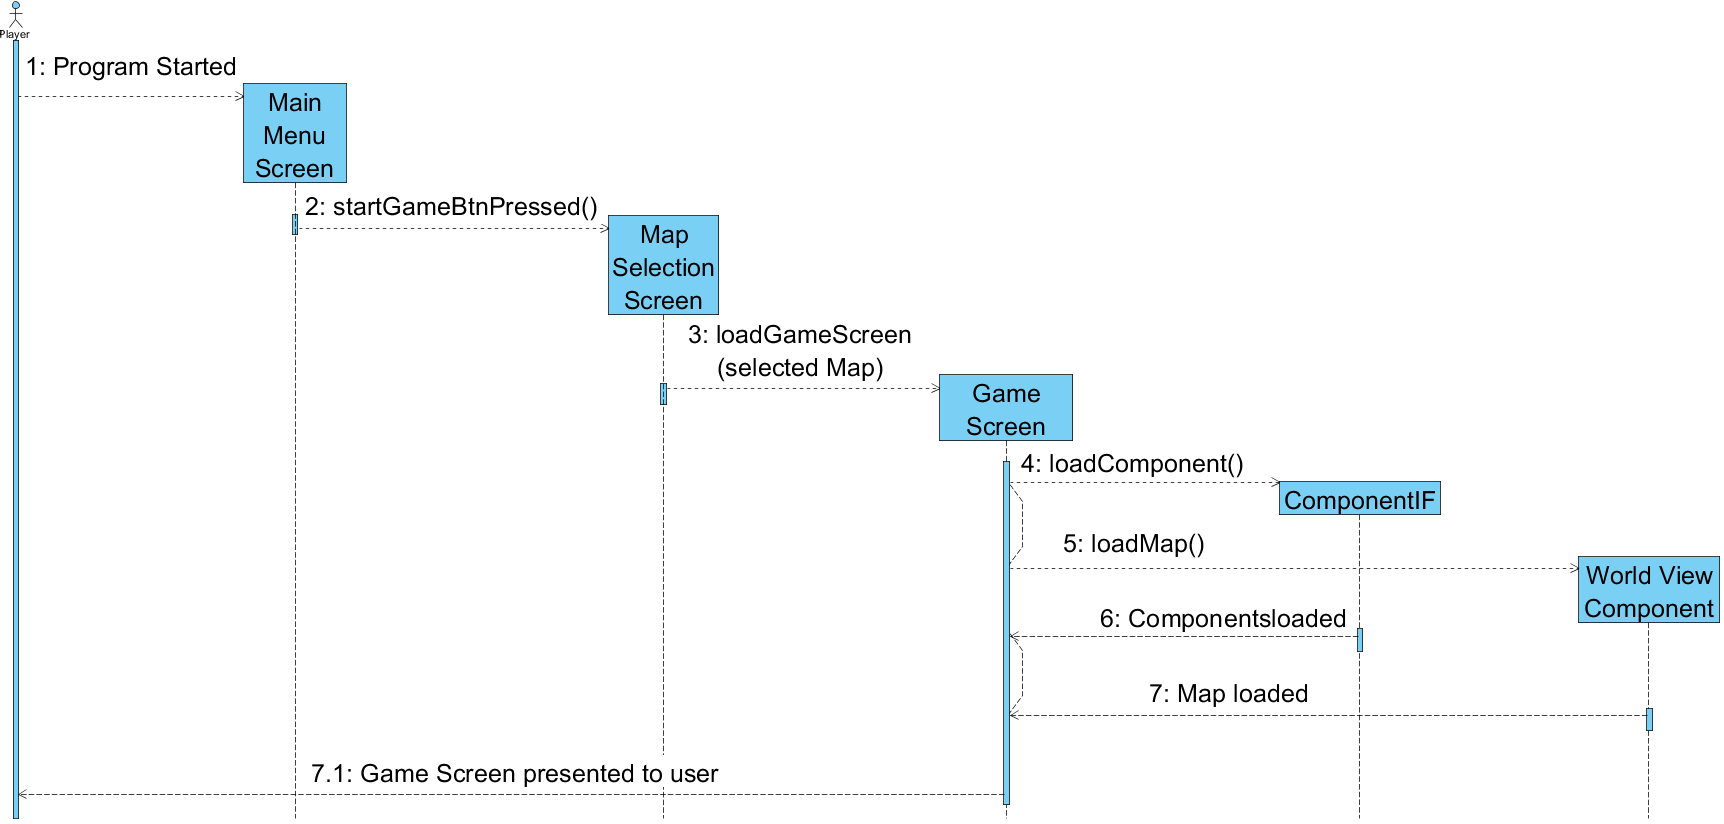
\includegraphics[width=12cm, origin=h]{images/Sequence-Diagram2.png}
		\\
		\caption{A sequence diagram drawn in Visual Paradigm}
	\end{center}
\end{figure}

\subsection*{Class Diagram}
The class diagram shows a detailed overview of the game and shows the relationships between different classes within the game.
\newpage
\begin{figure}[!h]
	\begin{center}
		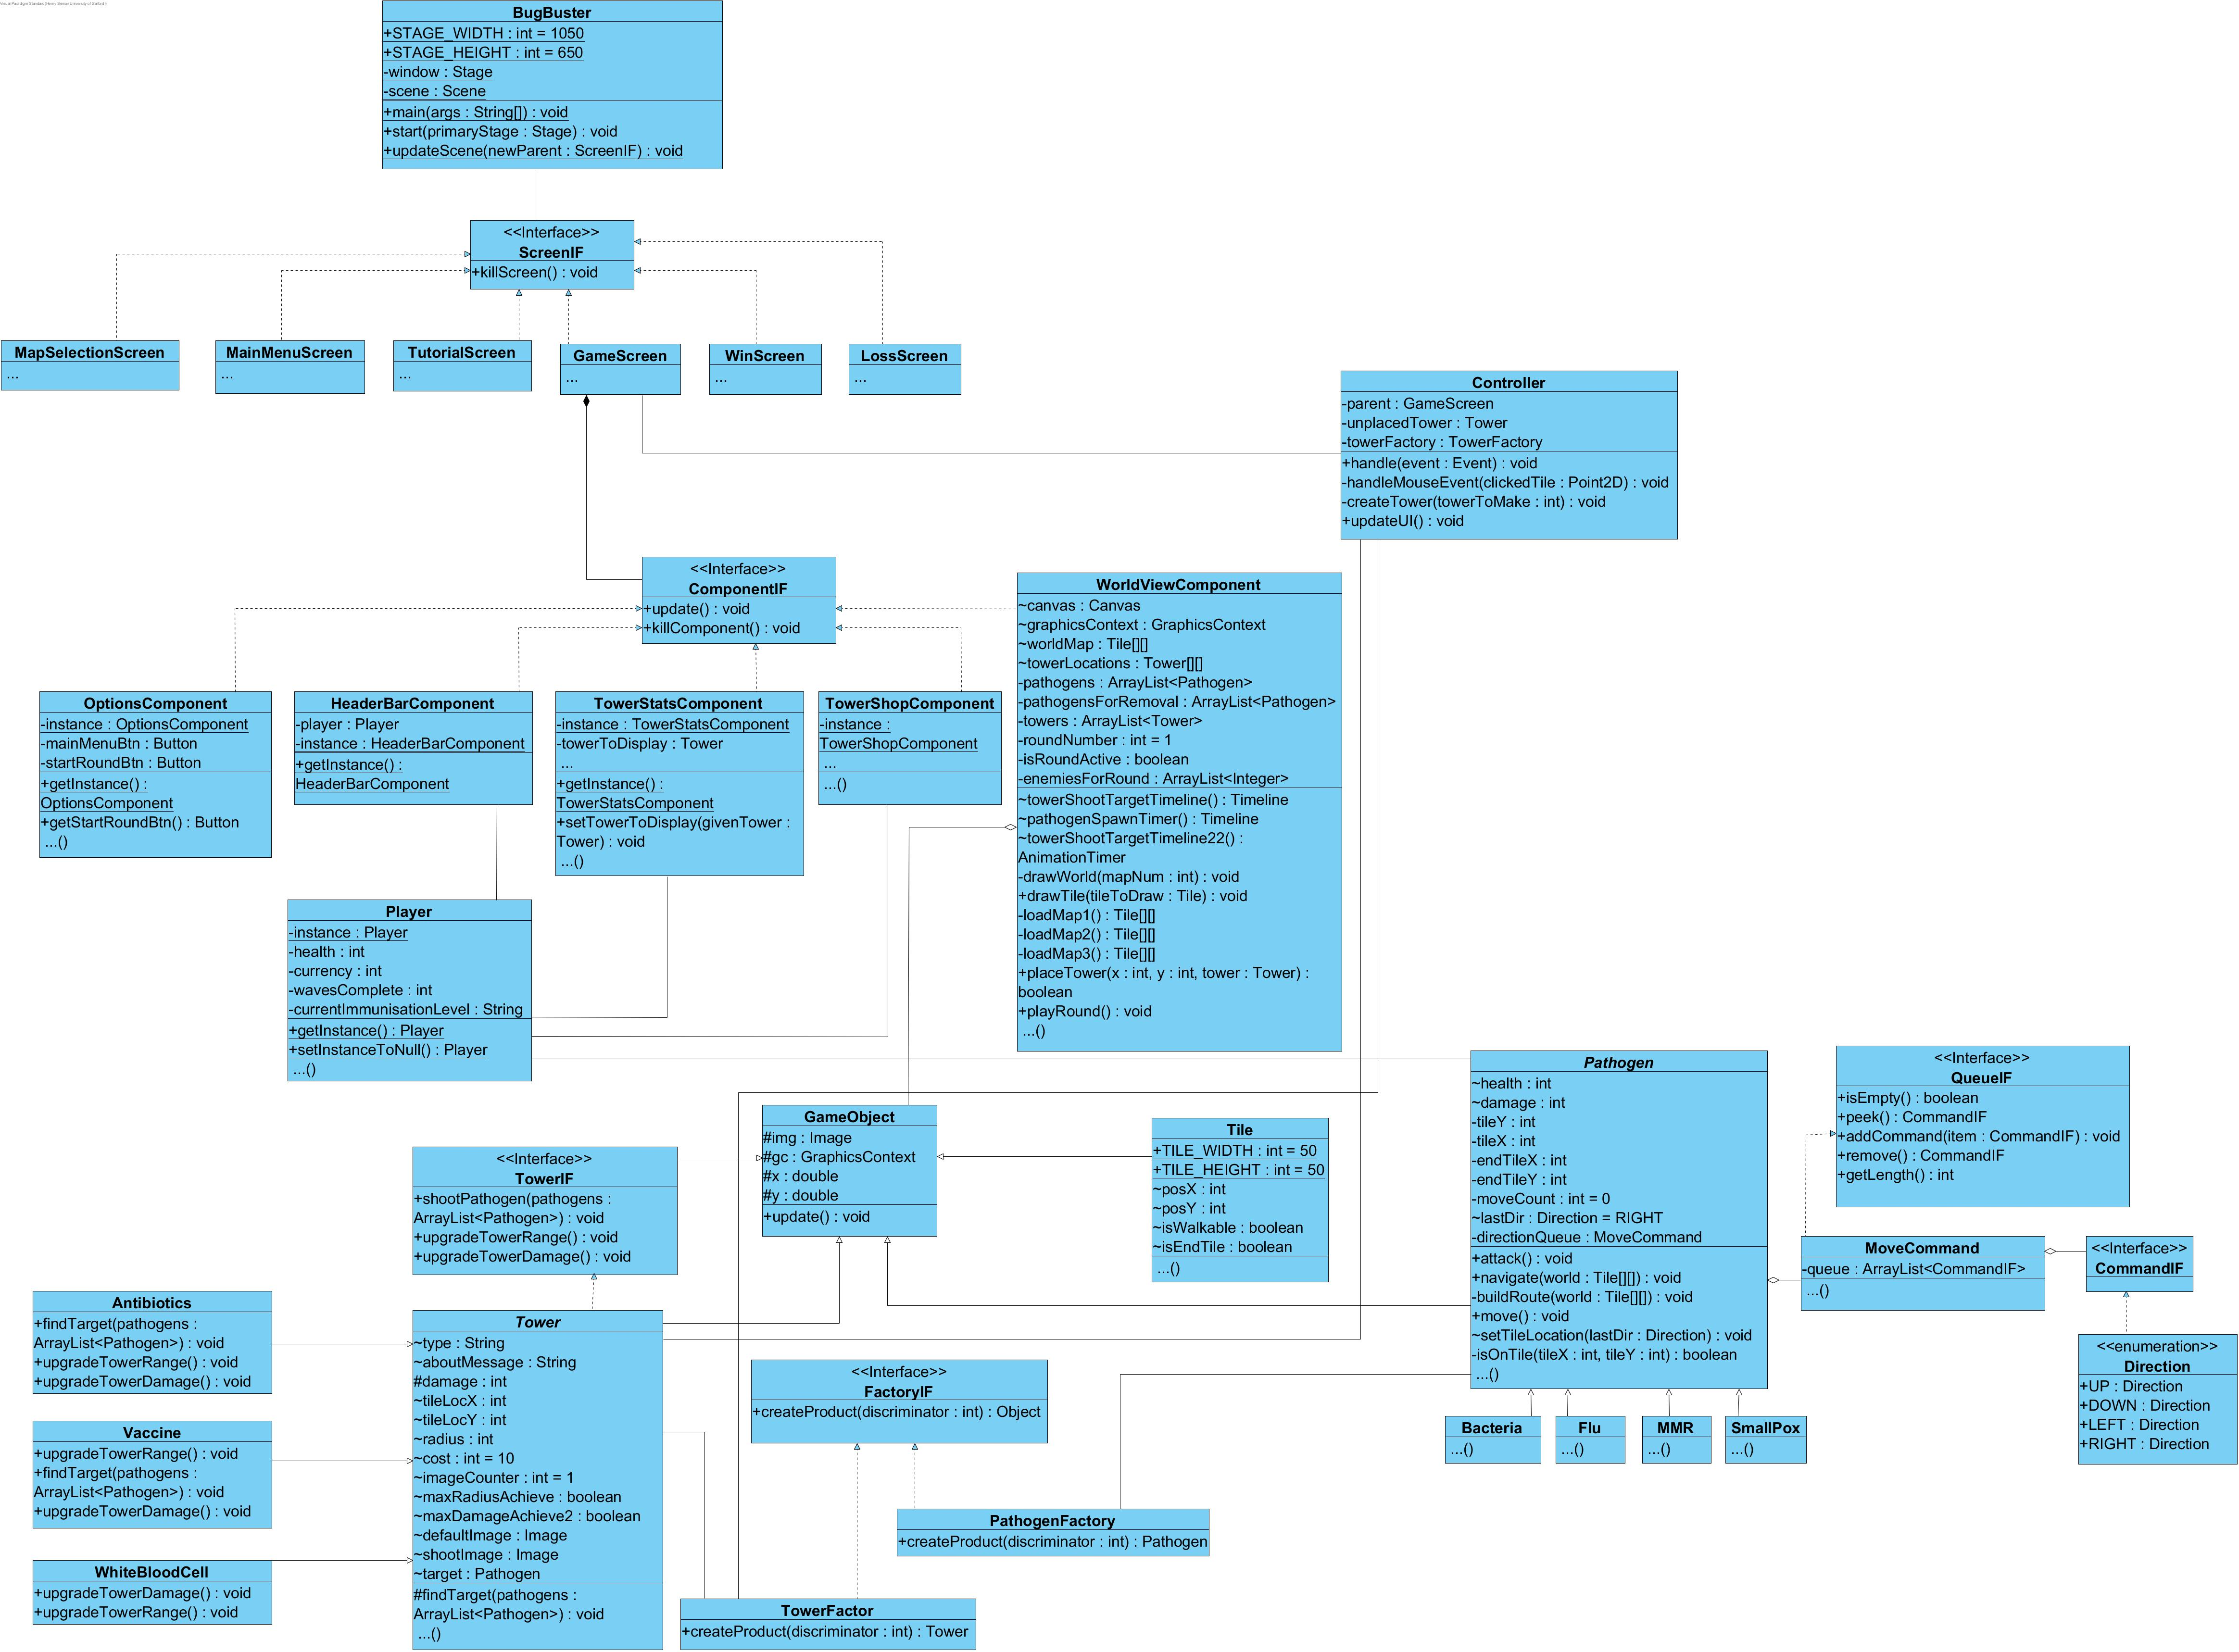
\includegraphics[width=23cm, angle=90, origin=h]{images/Class-Diagram.jpg}
		\\
		\caption{A class diagram drawn in Visual Paradigm}
	\end{center}
\end{figure}

\subsection*{Design Choices}
When designing the game, focus was placed on ensuring low coupling between the different classes that make up the game as well as ensuring high cohesion between an object and it's behaviours. This was a conscious choice that aimed to improve the \textit{`programmer experience'}.
\\
One of the design choices I made in order to achieve a good programmer experience was to break the sections of the user interface that are used by the GameScreen object into individual UI components. By providing the components with a common interface, \textit{ComponentIF}, I was able to ensure the components could be interacted with in universal ways therefore reducing the coupling within the user interface. This made it very easy to make changes to the user interface without those changes having effects on other portions of the interface. To make the separation of the user interface components and screens explicitly clear for future developers, the classes that inherrit from ComponentIF together are grouped in a package, alongside the interface. 

\section*{Design Patterns}
Design Patterns originate from structural architecture and refer to generalised solutions to common problems. It was found by Gamma \textit{et al} that a similar approach could be applied to object oriented software design. \cite{GoF-Book}. The software design patterns used in the project are outlined below, with detail and critique on the implementation.

\subsection*{Singleton}
The goal of the singleton design pattern is to ensure that only one instance of the object can exist at any given time, also ensuring that the object has a single point of global access \cite{GoF-Book}. The singleton design pattern is widely used within the project as there many objects of which only one needs to exist. By ensuring there is only once instance of any user interface components that make up the GameScreen object, the components become well encapsulated as well as more memory efficient. This feeds back into the \textit{`programmer experience'} as at any given time in development the programmer can be confident that only one instance of the object exists, meaning any change made to it will be processed by any other objects that interact with the singleton. Another advantage of implementing the singleton design pattern into the UI Components is that they can provide concrete implementations of the ComponentIF interface, something that would not be possible if they were static. 
\\
The singleton design pattern is also implemented in the player object. Throughout the game, only one player will be needed as it is only single player. Using a singleton design on the player stops an instance of the player having to be passed between different parts of the game, and allows the player to keep a strong encapsulation. Without using the singleton design, the player object would have to be static, which would limit further development as the player could not be treated as an object. There are instances where the player needs to be reset, such as the player dies and starts a new game. To accommodate for this event, the player class also includes a setToNull() method, which sets it's instance to null. This results in a new instance being created the next time an objects tries to access the player - resetting the field variables held by the player. 

\subsection*{Model View Controller (MVC)}
Originally created for use in SmallTalk, the MVC design pattern achieves the decoupling of the user interface and the logic of the program. In modern systems, MVC is common in web applications as it decouples the application in such a way that developers can apply their skills to the most applicable area (front-end developers work on the view whilst back-end developers work on the model). 
\\
The MVC design pattern was implemented into the game through the use of a controller object which handles events from UI Components. The MVC implementation used only decouples the events that span multiple user interface components. As some button events are simple, such as changing screen, it was felt that the system would have better cohesion if these events remained in their parent's class. 

\subsection*{Factory}
The Factory design pattern provides an abstract methodology for the creation of objects. Concrete implementations are then produced which meet specific requirements. This proves advantageous as it decouples the creation of an object from the object that needs access to it \cite{GoF-Book}.
\\
To incorporate a factory into the project, an abstract factory interface was produced, allowing method prototypes to be defined. Concrete definitions of the factory interface were developed to provide factory objects for creating both pathogens and towers. 
\\
The \textit{`programmer experience'} was greatly improved through the use of factories as it meant the towers and pathogens could change, but the way they were created and displayed on the screen for the player to interact with does not. 

\subsection*{Command and Marker}
The command pattern will encapsulate an operation as an object, which allows them to be stored as list of requests. More advanced implementations of this pattern allows for commands to be executed in reverse or `undone'. \cite{GoF-Book}
\\
A marker interface provides extra information about the object \cite{Lectures} and can be used as a sort of meta-tagging system. 
\\
The Pathogen class utilises the command pattern as part of it's path finding algorithm. Before a pathogen moves through the map, it searches for tiles which it can move to and builds a queue of movement commands that it will need to execute to move through the map. As the commands required by the pathogen are the directions it must take to navigate the map, the marker design pattern can be used to recast the direction as a command that requires execution. The implementation of these patterns provided a robust path finding algorithm that was well suited to the project.

\subsection*{Null Object with Delegation}
One design that was considered and then rejected was the use of the null object design pattern alongside the delegation pattern. The Null Object pattern allows an empty object to be created and used like a standard object, but the behaviours are overridden so they have no effect\cite{Lectures}. It would be feasible to delegate a pathogen to a null object pathogen when a tower kills the pathogen. The use of the null object pattern was rejected as it was not the most memory efficient solution. By adding a pathogen to a removal list once it was dead, and then removing it from the main pathogen list once that list had been iterated, the amount of memory the game used was reduced. This will provide the game with better performance and is a design choice that makes it more scalable. Through freeing up memory, it possible that more difficult rounds could have hundreds of enemies rather than tens of enemies. 

\section*{Future Improvements}
\subsection*{Interpreter Design Pattern}
In the current implementation, the map and the enemies that the player face are both hard coded into the game. Whilst this removes the need for map files, it tightly couples the map and rounds into the game's source code. A better design decision would have been to implement an interpreter design pattern. The interpreter pattern allows for a language to be defined alongside it's grammar using Backus-Naur Form\cite{GoF-Book}. These rules can then be used to interpret a string that follows these rules. Using the interpreter pattern it would be possible to decouple the map files and the enemies that are played each round to separate files. This would also allow for the users to create their own maps if they so wish. 

\subsection*{Prototype Design Pattern}
Through the implementation of a prototype design pattern, the game could clone instances of the bacteria pathogens as they move through the screen. This would help teach the end user that bacteria can multiply, but viruses cannot. The prototype design pattern allows for objects to be cloned and then edited\cite{GoF-Book} - which would allow for a bacteria object to be cloned, but be given a different graphic, signifying that it had been cloned. 

\section*{Conclusion}
Whilst the project was challenging, it provided a good learning experience. Through the production of an educational game, I was able to learn about design patterns within software architecture and experience first hand how different design choices made early on impact the project later on. 
This project has been the largest piece of software I have developed, but the use the design patterns and responsibility driven design made the process of going from assignment brief to final product very manageable. This has shown me how effective design patterns are as well as demonstrating the power of following good software practice, such as; lose coupling, high cohesion, and Parna's Principles. 

\bibliographystyle{agsm}
\begin{thebibliography}{9}
	\bibitem{GoF-Book}
	Gamma E, Helm R, Johnson R, Vlissides J. 2005. Design Patterns: elements of reusable object-oriented software. Addison Wesley.
	
	\bibitem{FizzBuzz}
	Henney K. 2017. FizzBuzz Trek HD. \url{https://www.youtube.com/watch?v=LueeMTTDePg}. Accessed December 2nd 2017.
	
	\bibitem{Lectures}
	Drumm, I. 2017. Software Architecture Lecture Notes. University of Salford
	
	\bibitem{UML-Distilled}
	Fowler M, Kendall S. 1999. UML Distilled: a brief guide to the standard object modelling language. 2nd Ed. Addison Wesley.
	
	\bibitem{background-sound}
	Background.mp3, Ben Sound, \url{https://www.bensound.com}
	
	\bibitem{laser}
	default-laser.mp3, Sound Bible, \url{http://soundbible.com/1087-Laser.html}
\end{thebibliography}

\end{document}          